In generale, il sistema consiste in una rete \textit{Peer-To-Peer} (\textbf{P2P}) che utilizza \textit{Proof-of-Work} (\textbf{POW}) per registrare l'elenco delle transazioni in un archivio pubblico, detto \textbf{blockchain}. Per una migliore comprensione del fenomeno si rimanda alla lettura dell'articolo originale di Satoshi Nakamoto \href{https://bitcoin.org/bitcoin.pdf}{Bitcoin}. 
L'implementazione del progetto è, almeno in parte, ripresa da quella descritta nell'articolo, fatta eccezione per lo sviluppodella POW, che segue i principi della criptovaluta \href{http://primecoin.io/bin/primecoin-paper.pdf}{\textbf{Primecoin}}.

In questa sezione sono enunciate le definizioni di transazioni (contenute in un blocco) e blockchain, e se ne discute la relativa implementazione. Sono poi elencate le definizioni delle altre componenti del sistema: il meccanismo di convalida di un blocco (la Proof-of-Work); il server Timestamp per la sincronizzazione oraria; il comportamento della rete all'avvio dell'esecuzione.

\subsection{Le transazioni e la catena di blocchi: la Blockchain}
La \textbf{blockchain} è una struttura dati ordinata, una lista concatenata di blocchi contenenti transazioni. L'intera struttura della blockchain può essere conservata in un file, oppure in un database. Un \textbf{block}, o blocco, è un contenitore, una struttura dati a sua volta, che aggrega transazioni che devono essere incluse in un \textit{ledger}\footnote{Il rermine ledger indica il libro mastro dei contabili, viene tradotto in italiano come registro.} pubblico e condiviso, la blockchain. 
Il blocco è composto da un \textit{header}, che contiene i \textit{metadata}, e dalla lista di transazioni che ne compongono la maggior parte della grandezza.

\subsubsection{Implementazione}

\subsection{Il Server Timestamp}
Un server timestamp offre un servizio che permette di conoscere l'ora esatta all'interno della rete. Un nodo che intende effettuare le operazioni di scrittura o di validazione di un blocco deve richiedere il \textbf{timestamp} al server. Esso garantisce l'esistenza dei dati al momento della richiesta.

\subsubsection{Implementazione}
In particolare, Jolie offre, tramite l'interfaccia \texttt{time} una \texttt{operation} che restituisce i millisecondi del \textit{current unix timestamp} nel momento esatto della richiesta. Tramite una chiamata a tale servizio si può ottenere il dato necessario da includere nel blocco. Qui è riportato un esempio si chiamata a tale operation, che può essere inserita in un server che accetta richieste e le inoltra al servizio time.
%
\lstinputlisting[language=Jolie]{code/timestamp.ol}
%

\subsection{La Proof-of-Work}
La PoW, è un algoritmo che viene utilizzato per raggiungere un accordo decentralizzato tra diversi nodi nel processo di aggiunta di un blocco specifico alla blockchain.
Tale algoritmo produce valori che vengono utilizzati per verificare che sia stata eseguita una notevole quantità di lavoro. Nell'immagine riportata qui sotto viene visualizzato un esempio di utilizzo di tecniche POW nel mondo delle criptovalute (in particolare quella di Ethereum ma generalizzabile a qualunque altra che usa POW).
\begin{center}
    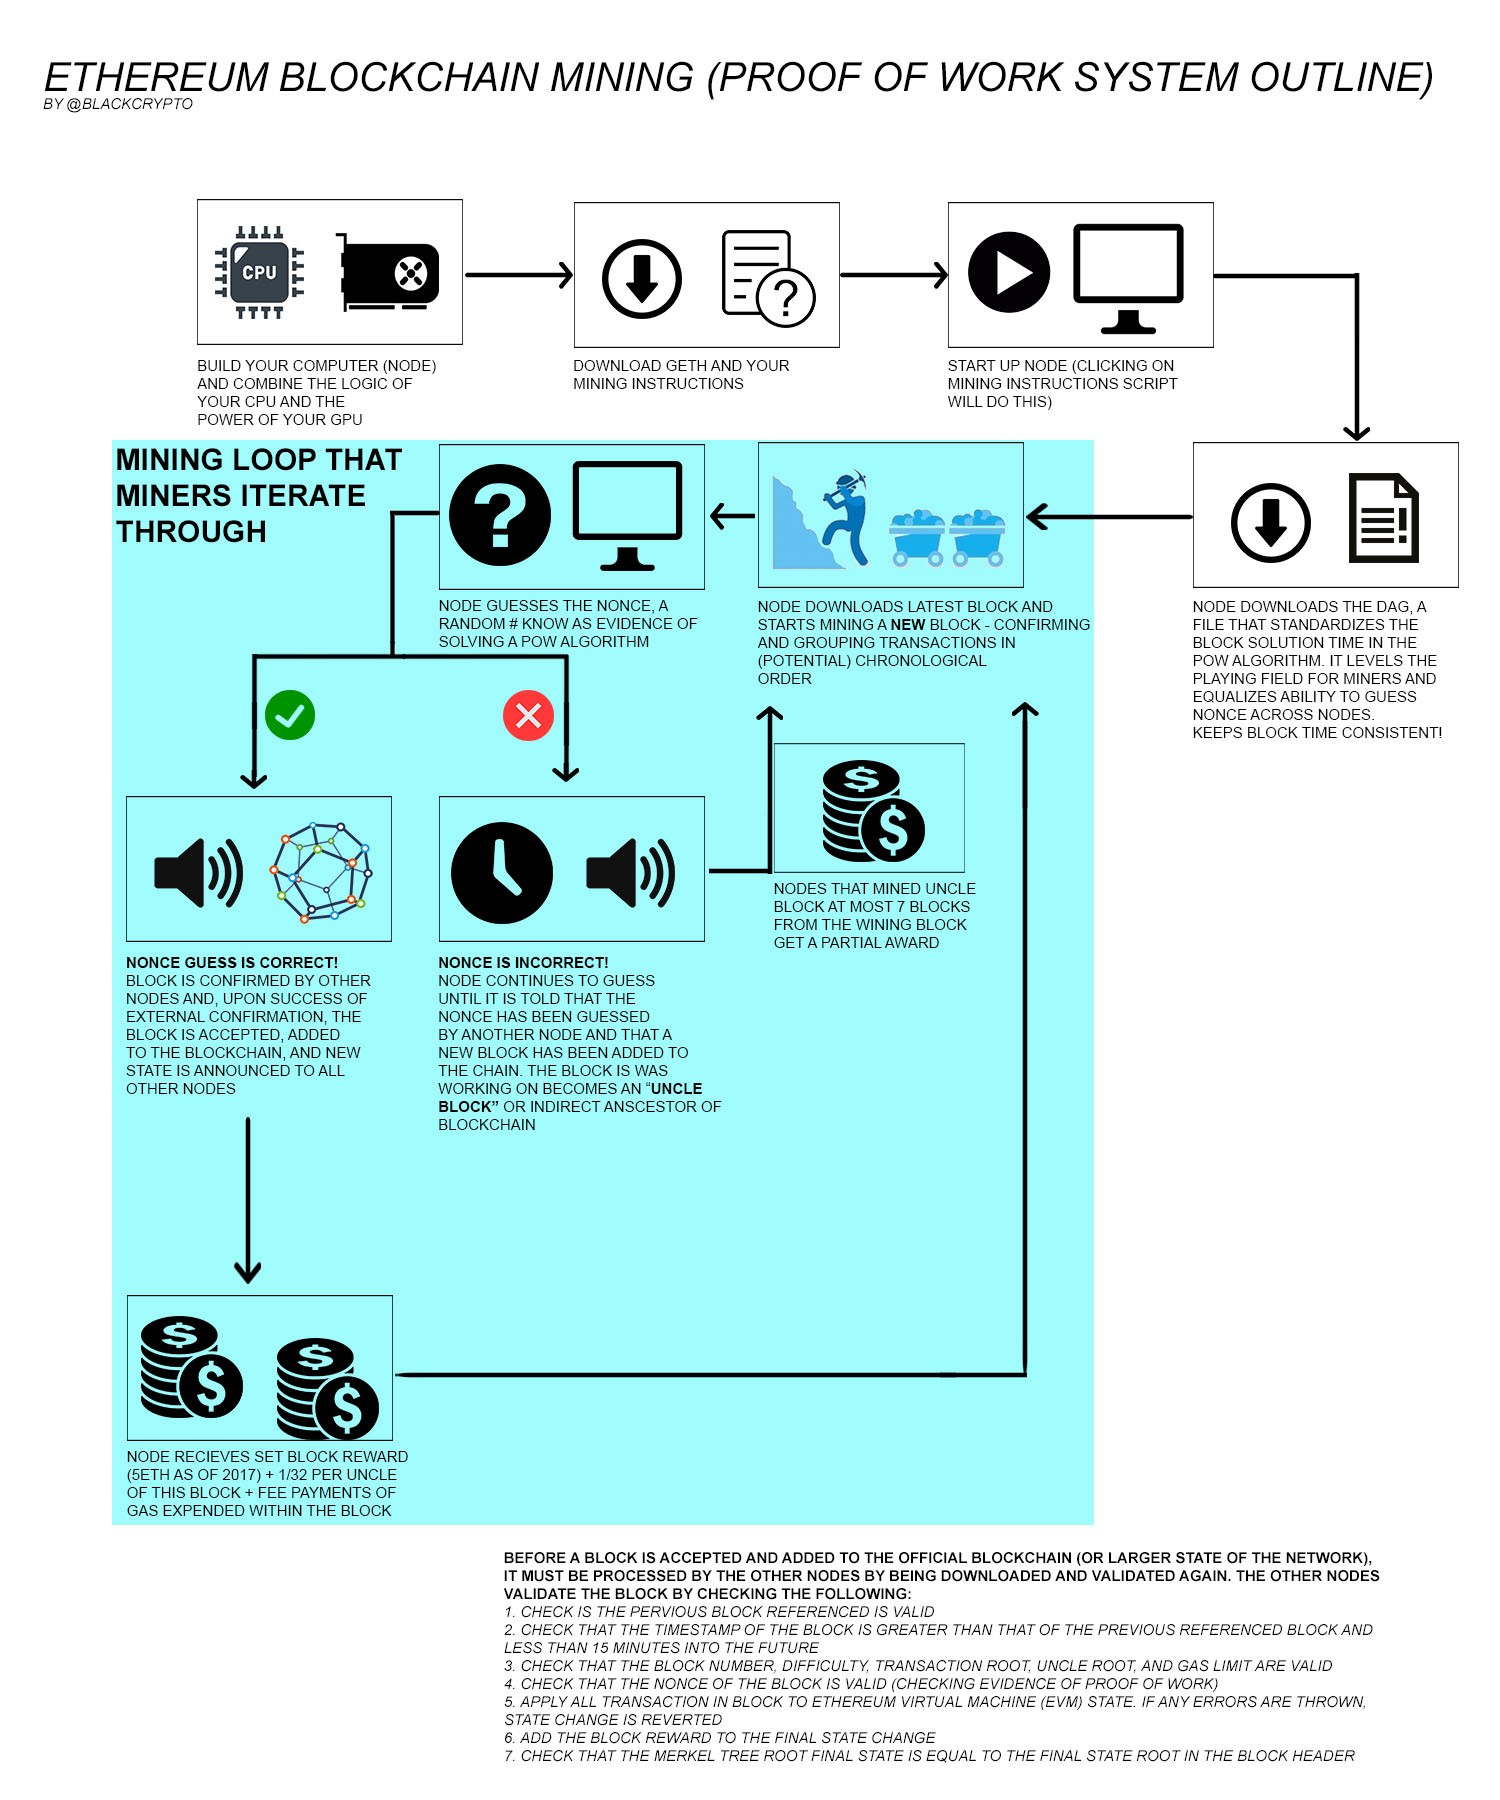
\includegraphics[width=\linewidth]{img/pow}
\end{center}

\subsubsection{Implementazione}
Per implementare un server timestamp basato su rete P2P, abbiamo bisogno di usare un sistema di proof-of-work\footnote{\url{http://www.wisdom.weizmann.ac.il/~naor/PAPERS/pvp.ps}}. Questo metodo consiste nell'obbligare i nodi che vogliono scrivere un blocco a cercare un valore che sia difficile da trovare e di cui sia facile controllarne la correttezza da parte degli altri nodi che vogliono validare la scrittura.
%
\begin{itemize}
    \item \textbf{Indice}: Un numero primo $p$ deve essere generato, una buona pratica sarebbe quella di generare un numero primo abbastanza grande, quindi si consiglia l'utilizzo di tipi \texttt{Long}. I \texttt{Long} in Java, quindi anche in Jolie, hanno un limite superiore pari a $9,223,372,036,854,775,807$. Oltre questo numero il sistema semplicemente termina di produrre prove.
    \item \textbf{Definizione}: $f_p(x) \equiv \sqrt{x} \bmod p$, cioè equivale ad estrarre tutte le radici quadrate modulo il numero primo $p$. Il dominio di $f_p$ è $\mathbb{Z}_p$.
    \item \textbf{Verifica}:  Dati $x,y$ controllare che $y^2 \equiv x \bmod p$.
\end{itemize}
%
Il meccanismo di controllo prevede solo una moltiplicazione, mentre non esiste un metodo veloce per l'estrazione delle radici modulo un numero primo, che non richieda meno di $\log{p}$ moltiplicazioni. Ne consegue che maggiore sia la lunghezza di $p$, maggiore sarà lo sforzo computazionale necessario, e quindi maggiore la differenza di tempo per valutare $f_p$ e per verificarne la correttezza.


\subsection{La Rete Peer-To-Peer}
Una rete P2P, come ad esempio quella di \href{www.emule-project.net/home/perl/}{Emule}, è una rete i cui nodi non sono \textbf{client} o \textbf{server} fissi, ma prendono forma di entità equivalenti o ``paritarie''.
\begin{center}
    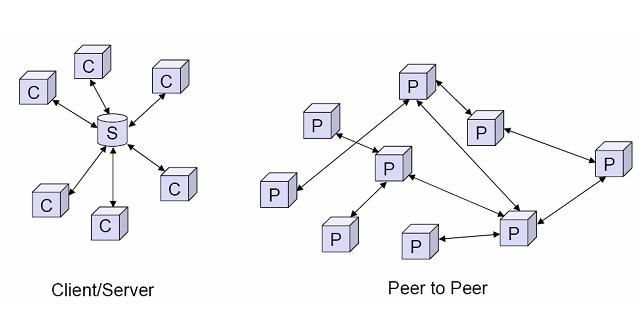
\includegraphics[width=\linewidth]{img/p2p}
\end{center}

\subsubsection{Implementazione}
L'esecuzione della rete P2P comprende i seguenti passaggi:
\begin{enumerate}
    \item Le nuove transazioni sono inviate in \textit{broadcast}\footnote{Nelle reti di calcolatori, il termine broadcast indica una modalità di instradamento per la quale un pacchetto dati inviato ad un indirizzo particolare (detto appunto di broadcast) verrà consegnato a tutti i computer collegati alla rete} a tutti i nodi che partecipano alla rete;
    \item Ogni nodo colleziona la nuove transazione in un blocco (una transazione per blocco!);
    \item Ogni nodo effettua del ``lavoro'' per provare di poter scrivere il blocco (POW);
    \item Quando un nodo trova una prova, invia il blocco in broadcast a tutti i nodi;
    \item I nodi accettano il nuovo blocco solo se la transazione contenuta in esso è valida e non è stata già ``spesa'';
\end{enumerate}

I nodi considerano sempre la blockchain più lunga come quella corretta. Nel caso in cui due nodi inviano versioni differenti del nuovo blocco contemporaneamente, alcuni nodi potrebbero riceverne  una versione, altri l'altra. In quel caso il nodo lavora sul blocco ricevuto temporalmente prima. Il nodo che ha lavorato su un blocco non sincronizzato se ne rende conto quando una nuova validazione viene richiesta, in questo caso egli manda in broadcast una richiesta di sincronizzazione sul blocco in questione e, una volta ricevuta risposta, aggiorna la blockchain alla versione più recente, potendo così validare il nuovo blocco ricevuto.

\subsection{Il Network Visualizer}
Il Network Visualiser è un tool amministrativo da terminale per il monitoraggio del sistema.

\subsubsection{Implementazione}
%
